\chapter{Company Profile}

This chapter describes the customs and culture of Kaz Software.
Each section describes the overview of Kaz Software, the way it operates, what services they provide, technology used here, key features, location and what people here does for recreation. 

\section{Company Overview}

Kaz Software is one of the best and most experienced software company in Bangladesh.
It started as a start-up software outsourcing company in \textcolor{red}{8 June, 2004} and became a limited company in 2005 and continued to develop year after year.
Typically Kaz Software builds software for the clients, but sometime they would be doing something completely different like researching business data or setting up their firewall.
Kaz Software has some really talented engineers, designers, and content specialists to give it's clients a well built software.

\begin{figure}[h]
    \begin{center}
        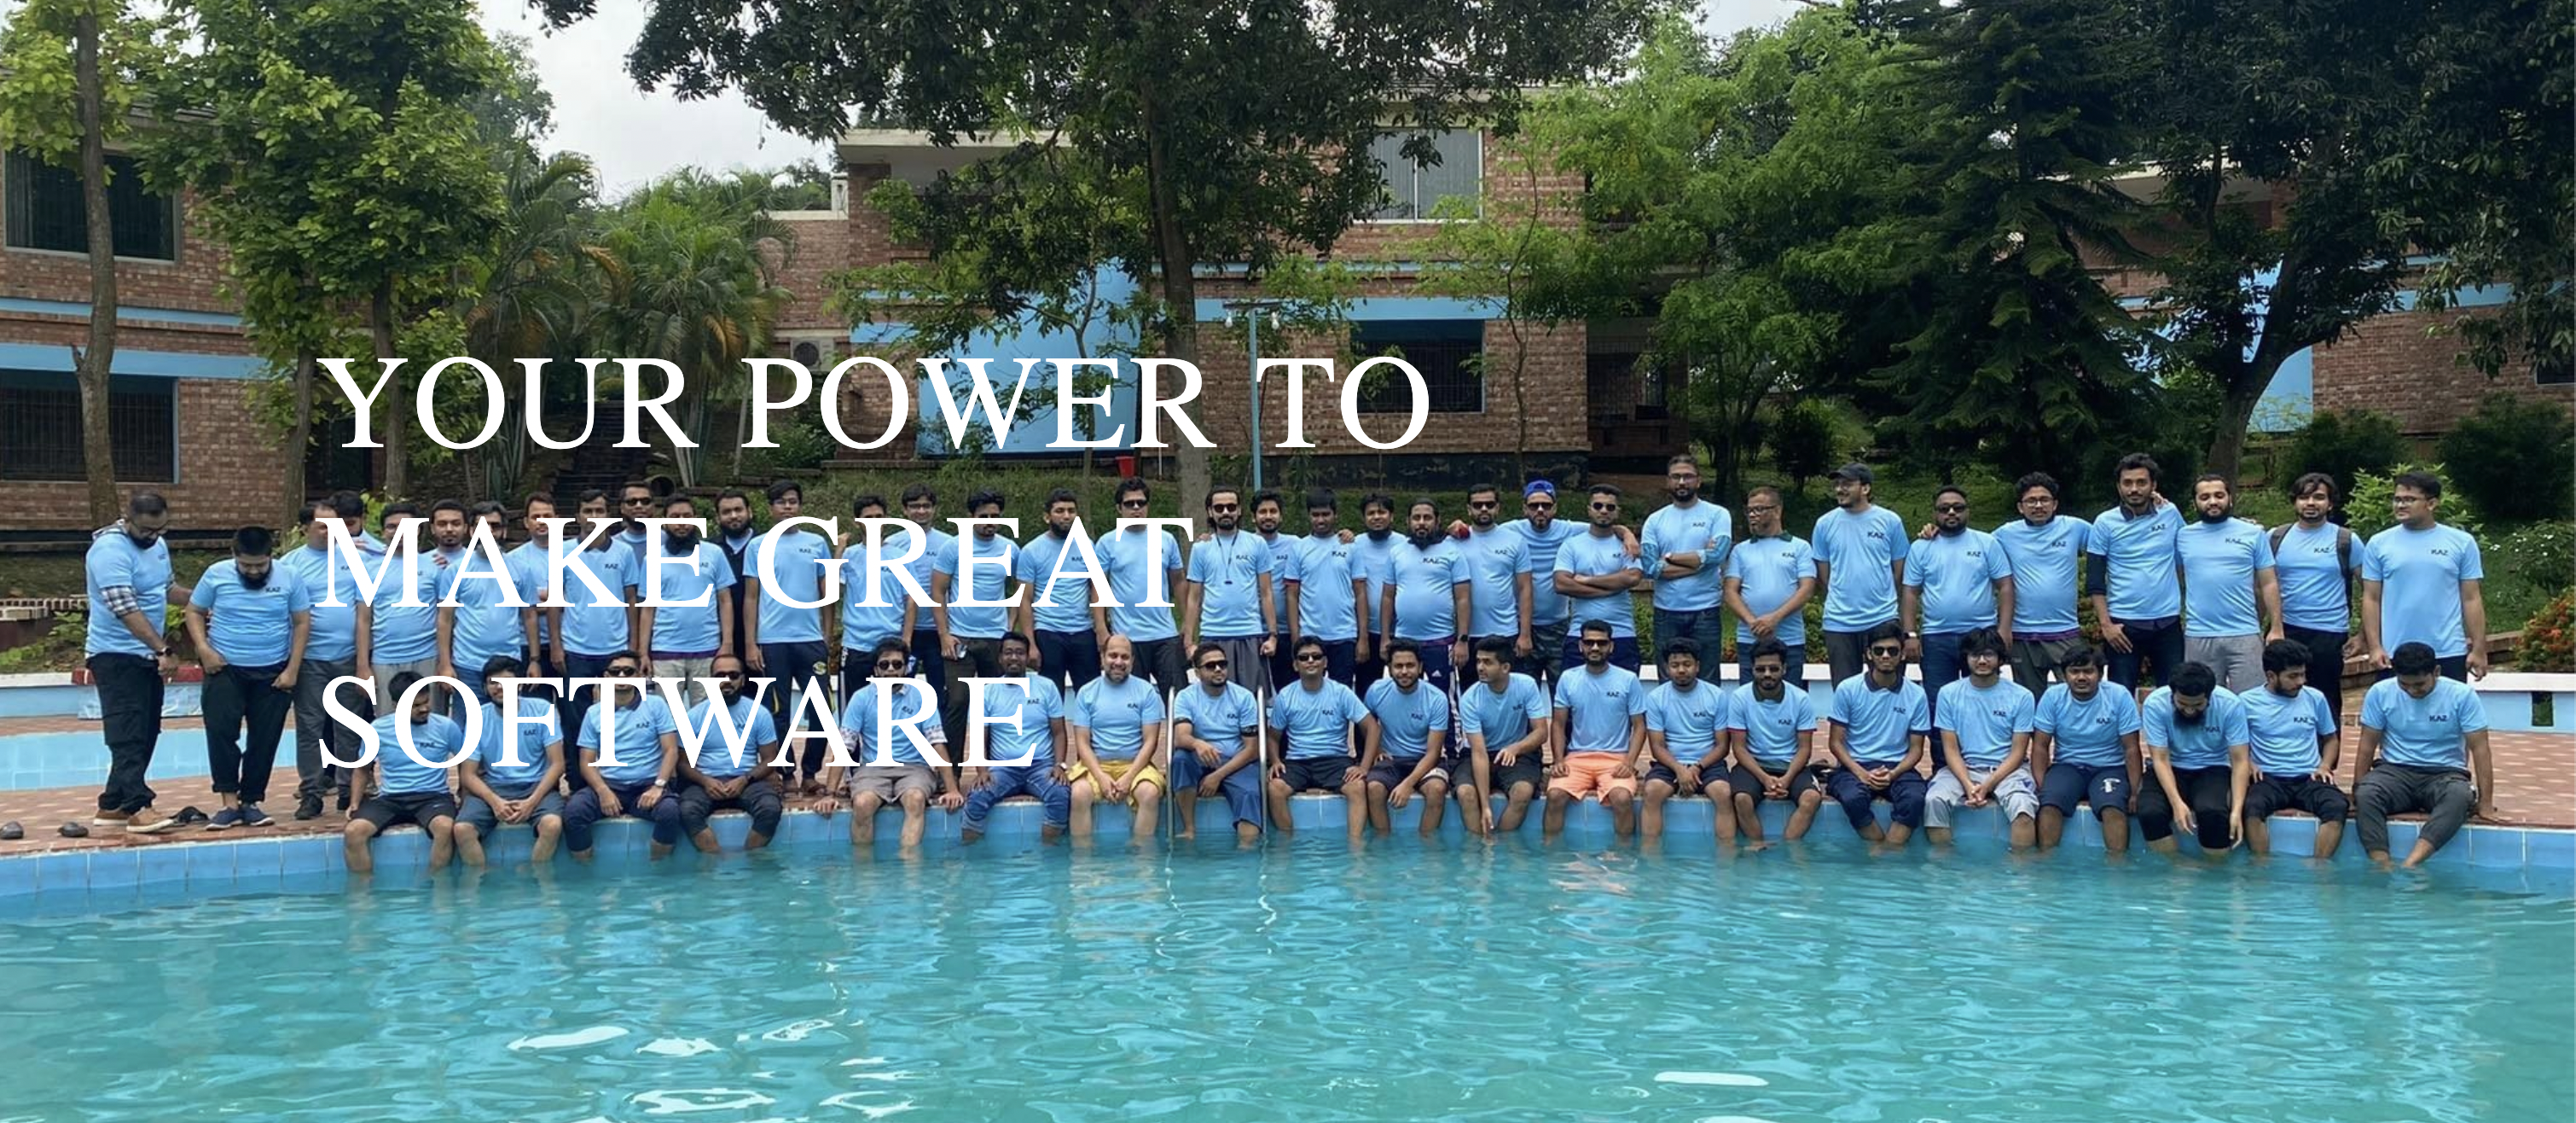
\includegraphics[width=0.9\textwidth]{images/Chapter2/cto_tour.png}
        \label{fig:CTO_Tour}
    \end{center}
\end{figure}

\section{Leadership}

An organization will not be able to operate for more than 18 years, if it does not have experienced and passionate people in the leadership roles.

\subsection[Founder and CEO]{Wahid Choudhury (Founder and CEO)}

Wahid has more than 20 years of experience in software development.
He is the founder and leader of several software companies in diverse industries such as regulatory compliance, eCommerce, legal services and computer games. 
Wahid has an exceptional technical background, as well as the advantage of having worked with dozens of start-ups during all stages of their technical and business development. He founded his first software company, Kaz Software, in 2004.

\subsection[CTO]{Shawal Siddique (CTO)}

Shawal is a technology leader and has more than 15 years of experience in software development space.
His strength in technical project is over a wide range of projects in device drivers, enterprise web applications and mobile apps using technologies such as Asp.NET, Asp.NET Core, .NET Core, Xamarin, Angular, Aurelia, Angular JS, Knockout JS, Node JS, Azure and AWS.

\subsection[Adviser]{Hafiz Choudhury (Adviser)}

Hafiz is an international tax consultant and entrepreneur.
He works with major multinationals on tax policy and business strategy issues; he also advises governments on tax policy and administration through his consulting firm, The M Group, Inc.

\section{Services}

Kaz Software offers software development and content management services to international customers across multiple industries.
Kaz understands the challenges that its customers face within and across these industries.
Kaz provides practical, pragmatic and powerful solutions to address those challenges.

\begin{figure}[h]
    \begin{center}
        \includegraphics[width= 0.8\textwidth]{images/Chapter2/kaz_services.png}  
        \label{fig:kazServices}
    \end{center}
\end{figure}

The services of Kaz Software covers every step of software development, from ideation to delivery.

\subsection{Ideation, Graphics and Interaction Design}

The design team in Kaz software helps the clients through the digital design and strategy maze.
They work through every stages of a project with the client and keep brainstorming and create mockups, demos and presentations.
And during interaction design, Kaz Software always prefer to create the simplest solution.

\subsection{Software Development}

Teams at Kaz Software help our customers build  customized software - everything from web to desktop to enterprise to mobile and beyond. 
They have been building softwares for various industries since 2004 and worked with many technology platforms and have collaborated with many teams over these years. \\

Kazians have worked on web applications, created desktop applications, and built numerous mobile applications. Some of things that they have built:

\begin{enumerate}
    \item Social app with localization
    \item Desktop based tax optimization tool
    \item Corporate data management application
    \item Document repository
    \item Database driven file system
    \item Content rich web application
    \item LDAP management tool
    \item iPhone/Android/Windows mobile applications
    \item Online holiday management tool
    \item Location content service
    \item Location based social app platform
    \item Flex based visio like diagramming tool
    \item Desktop based diagramming and layouting tool.
    \item Symbian application
    \item VoIP billing solution
    \item Mobile content solution
    \item Stock trading portal
    \item International trade research and management tool
\end{enumerate}

Kazians don't specialize in particular technologies, but they are definitely proficient ein wide array of tools and systems.
Every product is unique, and they try to fit the right skills for that particular product.

\subsection{Quality Assurance}

Integrated quality assurance approach of Kaz Software incorporates aspects of agile and lean development with the stability and reliability of traditional SQA process.
They believe software quality assurance is only possible with a mixed set of procedures which should involve all members of the team collaborating with a dedicated team of SQA professionals.
Because of their involvement with all kinds of projects their SQA teams are exposed to a variety of technology and business domains.
Types of testing services Kaz Software provides:

\begin{enumerate}
    \item Product testing
    \item Performance and Load testing
    \item Content Validation Testing
\end{enumerate}

\subsection{Data, Content and Research}

Kazian research teams have researched, compiled and maintained content in diverse fields and for a variety of applications.
The research team is supported by our data specialists who leverage technology to optimize data gathering and ensure that the data is stored and managed efficiently.
Services provided on this area by Kaz Software:

\subsubsection*{Research}

\begin{enumerate}
    \item Research and compile information
    \item Categorize existing content
    \item Meta tag content
    \item Search and collect publicly available documents
    \item Professional domain based translation of information
    \item Statistical and economic analysis
    \item News gathering and summarizing
\end{enumerate}

\subsubsection*{Create and Maintain}

\begin{enumerate}
    \item Write, edit, proof read content
    \item Maintain content in blogs, CMS or other systems
    \item Translate existing content
    \item Create and maintain structured content like spreadsheets
    \item Maintain newsletters/news services
\end{enumerate}

\subsubsection*{Data Services}

\begin{enumerate}
    \item ransformation of existing data to and from various formats such as csv, xml, etc.
    \item Extracting data from unstructured or structured sources
    \item "Cleaning" data by removing errors, unwanted information etc.
    \item Storage solutions - Databases, XML, flat file
\end{enumerate}

\section{Human Resource}

Kaz has 110+ employees at this moment and they are planning to recruit more.
Since the beginning, Kaz has grown in numbers of resources and production every year.
Kaz doesn't hire developers, designers or QA engineers.
Kaz hires people who solve problems.
And it hires only the best.
Kaz runs regular training and review sessions to keep it on the top.

\section{Facilities for Employees}

Kaz Software always keeps the happiness of their employees at the top priority.
As a result they provide a lot of facilities to keep the Kazians happy.

\subsection{Friendly Environment}

Kaz Software is like one big Family.
Work is fun here.
The work environment here is friendly, informal, fun and knowledge oriented.
Chain of command is not followed here.
Employees consider the company to be their own responsibility.

\subsection{Vacation and Optional WFH}

Kaz Software provides 17 days of paid vacation per year. 
A Kazian can take a full day or half day leave anytime, until it exceeds total of 17 days per year.\\

Another great initiative by Kaz Software is an employee can either go to office or work from home, it's up to them.
And any kind of technical support will be provided no matter where you are, home or office.
Although working from office is more fun because of the friendly environment.

\subsection{Lunch and Snacks}

Kaz Software does not provide any lunch or snacks except tea and coffee.
An employee can go and make their own tea or coffee or ask a Shoinik to make them one.

\subsection{Indoor and Outdoor Games}

Almost every Kazian is a cricket lover.
They play short-pitch cricket every working day after lunch, in the office premises.
There is a table tennis board in the ground floor and Kazians can play anytime they want.

\textcolor{red}{\LARGE Images Goes Here}

\subsection{Recreation}

Kaz has different ways for recreation of employees.
Release parties, picnics, ’Hudai party’, and outings are part of it.
Every year in December Kaz organizes their anniversary party.
Which is either taking all of the employees for an international trip, or a 7 to 10 days trip inside Bangladesh.
And this is fully paid by the office.
In spite of being an intern, I received all these facilities and consider myself lucky.

\subsection{Bonuses and Increment}

Kaz Software does not provide any festival bonus.
But they provide a bonus equal to the salary of a employee after every anniversary of their joining and they get a increment of 10 to 15 percent of their current salary.
This may vary according to an employee's performance.